\documentclass{standalone}
\usepackage{tikz}
%x code={
\usetikzlibrary{positioning}
%x }
\usetikzlibrary{decorations.pathreplacing}

\begin{document}

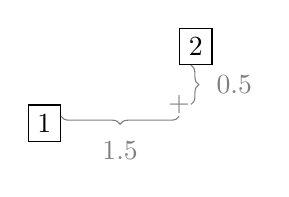
\begin{tikzpicture}
%x description="nodes with relative positioning"
%x code={
	\node[draw] (a) at (0,0) {1};
	\node[draw] (b) [above right=0.5 and 1.5 of a] {2};
%x }

\tikzset{brace/.style={decorate, decoration={brace, amplitude=0.1cm}, gray}}
\draw[brace]
	(a.north east) ++(1.5,-0.15)
	-- node [below=0.2] {1.5}
	+(-1.5,0);

\draw[brace]
	(b.south west) ++ (0.15,0)
	-- node [right=0.2] {0.5}
	+(0,-0.5);

	\node[gray] at (a.north -| b.west) {+};

\end{tikzpicture}

\end{document}
